% !TEX program = xelatex
\documentclass[20pt, a4paper]{article}
\usepackage{listings}
\usepackage{hyperref}
\usepackage{tikz}
\usetikzlibrary{arrows, shapes, automata, petri, positioning, calc}
% Justify paragraphs
\usepackage{graphicx}
\usepackage{ragged2e}
\usepackage{color}
\usepackage{xepersian}
\usepackage{subfiles}
\settextfont[Scale=1]{XB Roya}
\renewcommand{\baselinestretch}{1.5}

\begin{document}
\centerline{الگوریتم‌های موازی}
\centerline {خانم دکتر دامرودی}
\centerline{علیرضا سلطانی نشان}
\centerline{\today}

\tableofcontents

\section{مفاهیم اولیه}

نگارش این بخش تکمیل نشده است.

\section{وابستگی‌ها}

هیچ برنامه‌ای نمی‌تواند سریع‌تر از برنامه‌ای که مدت زمان بیشتری، زمان رسیدن به
نتیجه را سپری می‌‌کند، اجرا شود. زیرا محاسباتی که نسبت به محاسبات قبلی به
یکدیگر، در زنجیره‌ای از فرایند‌ها وابستگی دارند، باید به ترتیب اجرا شوند چرا که
به صورت سریالی می‌باشند.  همه الگوریتم‌ها شامل وابستگی‌هایی هستند که می‌توان
آنها را تشخیص و به صورت مناسب آنها را حذف کرد تا بتوان محاسبات مستقل به صورت
موازی را حل کرد.

\subsection{انواع وابستگی‌های داده}

وابستگی‌های داده به سه دسته زیر تقسیم می‌شوند:

\begin{enumerate}
    \item \lr{Data Flow Dep \footnote[1]{Dependency}} ماهیت برنامه
    \item \lr{Anti Data Dep} برنانویس
    \item \lr{Output Data Dep} برنامه نویس
\end{enumerate}

\subsection{منبع} 

اگر دو دستورالعمل بخواهند به صورت همزمان کار کنند، به گونه‌ای که روی یک منبع
عملیات خواندن و نوشتن را انجام دهند، دو حالت به وجود می‌آید:

\begin{enumerate}
    \item یا در ماهیت خود برنامه وجود دارند
    \item یا برنامه نویس ایجاد می‌کند که قابلیت حذف دارد
\end{enumerate}

نکته: یکی از وظایف اصلی کامپایلر حذف وابستگی‌هایی است که برنامه نویس ایجاد
می‌کند و قبل از مرحله اجرا انجام می‌شود و باعث کارایی بالا برنامه می‌شود.

% TODO: Should fix by a simple diagram

وابستگی‌های زیر را در نظر بگیرید:

S[i]: O ... = .... O

S[j]: O ... = .... O

\subsection{وابستگی \lr{WBR} یا \lr{Write Before Read}}

این وابستگی در ابتدا روی متغیر مورد نظر داده‌ای را می‌نویسد و سپس آن را در
فرایندی دیگر می‌خواند. به این نوع از وابستگی، وابستگی \lr{Date Flow} گفته
می‌شود.

برای مثال:

\begin{enumerate}
    \item s[i]: A = B + C , s[j] K = A + C
    \item s1: A = B + C , s2: E = A - D
\end{enumerate}

\subsection{وابستگی \lr{RBW} یا \lr{Read Before Write}}

در این از وابستگی در ابتدا عملیات نوشتن روی متغیر صورت می‌گیرد، سپس از آن متغیر
برای خواندن مقدار استفاده می‌کند. به این نوع از وابستگی \lr{Ani Data}

برای مثال:

\begin{enumerate}
    \item s[i]: B = C + A , s[j]: A = K + J
    \item s[i]: B = A * D , s[j]: A = F - 5
\end{enumerate}

\subsection{وابستگی \lr{WBW} یا \lr{Write Before Write}}

این نوع از وابستگی به شکل خطی می‌باشد. یعنی در مرحله اول فرایند ابتدا بر روی آن
مقداری می‌نویسد، سپس مجددا این عمل را تکرار می‌کند. به این نوع وابستگی
\lr{Output Data} گفته می‌شود.

برای مثال:

\begin{enumerate}
    \item s[i]: A = B + C , s[j]: A = K + J
    \item s[1]: A = B + C , s[2]: A = D + E
\end{enumerate}

نکته: برای نمایش وابستگی‌ها از گراف استفاده می‌کنند.

نکته: اگر تمام مسیر‌های گراف به یک جهت باشد (هم جهت باشد) و حلقه وجود نداشته
\footnote{Performancee} باشد، گراف مورد نظر به شکل آبشاری خواهد بود. که در این
حالت می‌توان با اجرای مناسبی پردازشی را انجام داد.

% TODO: شکل مربوط به نوع هر وابستگی یعنی یال‌ها کشیده شود

نکته: نتیجه وابستگی‌ها به شکل جدول وابستگی‌ها یا \lr{Dependencies table} نشان
داده می‌شود.

% شش حالت استیت‌ها رو بکش و با دپس مناسب به هم وصل کن

\footnote{\lr{Scaler 3 of (5, 2) Vector => (15, 6)} یادآوری:}

% TODO: مسئله و گراف وابستگی اول نوشته شود.

در وابسته اول، مهم‌ترین نکته در آن است که بایستی ارتباطات حداقل دو اندیس را در
نظر داشته باشیم تا بتوانیم وابستگی مورد نظر را پیدا کنیم. برای مثال در این
وابستگی در صورتی که تنها روی یک اندیس به دنبال وابستگی بگردیم نمی‌توانیم حلقه را
پیدا کنیم. در صورتی که در ذات این برنامه حلقه یا وابستگی نوع \lr{Output date
deps} وجود دارد.

% TODO: مسئله و وابستگی دوم نوشته شود.

% TODO: مسئله و وابستگی سوم نوشته شود

% TODO: مسئله و وابستگی چهارم نوشته شود

نکته: هر چقدر تنوع بیشتری در متغیر‌ها وجود داشته باشد، وابستگی نیز کمتر می‌شود
(فضیه گوناگونی متغیر).

\subsection{انواع ایجاد وابستگی}

حلقه‌ها در برنامه به دو شکل هستند:

\begin{enumerate}
    \item \lr{Do All}: همه اندیس‌ها در دستورالعمل‌ها یکسان است.
    \item \lr{Do Across}: اندیس دستورالعمل‌ها متفاوت است.
\end{enumerate}

نکات:

\begin{enumerate}
    \item متغیرهای اسکالر باعث ایجاد وابستگی بین تکرار‌های مختلف می‌شوند
    \item در حلقه \lr{Do All} به دلیل یکسان بودن اندیس‌ها وابستگی ایجاد نمی‌شود.
    \item در حلقه‌های \lr{Do Across} به دلیل تولید اندیس مختلف به ازای لیست‌ها،
    باعث ایجاد وابستگی به صورت تو در تو می‌شود. مهم ترین مثال این حلقه‌ را
    می‌توان به عامل دستورالعمل \lr{A[i] = A[i + 1] / C} و مانند آن اشاره کرد.
    \item وابستگی \lr{Data flow} کاملا به ذات برنامه مربوط است اما وابستگی‌های
    \lr{Anti data} و \lr{Output data} به دلیل عدم رعایت اصول موازی سازی توسط
    برنامه نویس در برنامه ایجاد می‌شود.
\end{enumerate}

\subsection{حذف وابستگی}

سه روش برای حذف وابستگی وجود دارد:

\begin{enumerate}
    \item \lr{Variable renaming}
    \item \lr{Scaler expansion}
    \item \lr{Node spliting}
\end{enumerate}

\subsubsection{حذف وابستگی با روش تغییر نام}

در مثال زیر دستورالعمل‌های زیر را خواهیم داشت:

\begin{LTR}
    \begin{enumerate}
        \item A = B * C
        \item D = A + 1
        \item A = A * D
    \end{enumerate}
\end{LTR}

% TODO: دیاگرام این مسئله را بکش.

همانگونه که در صفحه پیشین گفته شد، هر چقدر تعداد متغیر‌های مختلفی داشته باشیم
باعث می‌شود تا وابستگی کمتری در برنامه داشته باشیم.

در این مسئله در متغیر \lr{A} برای بار دوم عمل نوشتن صورت گرفته است. پس به همین
خاطر بایستی دستورالعمل سوم را تغییر نام دهیم تا بتوانیم کمترین وابستگی را داشته
باشیم.


\begin{LTR}
    \begin{enumerate}
        \item A = B * C
        \item D = A + 1
        \item AA = A * D
    \end{enumerate}
\end{LTR}

% TODO: دیاگرام این مسئله را بکش.

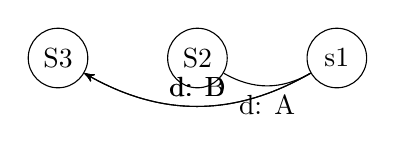
\begin{tikzpicture}[node distance=2cm and 1cm,>=stealth',auto, every place/.style={draw}]
    \node [place] (S1) {s1};
    \node [place] (S2) [left=of S1] {S2};
    \node [place] (S3) [left=of S2] {S3};

    \path[-] (S1) edge [bend left, below] node {d: A} (S2);
    \path[->] (S1) edge [bend left, above] node {d: B} (S3);
    \path[->] (S1) edge [bend left, above] node {d: D} (S3);
\end{tikzpicture}

% \begin{tikzpicture}[node distance=2cm and 1cm,>=stealth',auto, every place/.style={draw}]
%     \node [place] (S1) {S1};
%     \coordinate[node distance=1.1cm,left of=S1] (left-S1);
%     \coordinate[node distance=1.1cm,right of=S1] (right-S1);

%     \draw[->, thick] (left-S1) -- (S1);

%     \node [place] (S2) [right=of S1] {S2};
%     \node [place] (S3) [node distance=1.5cm,below =of right-S1] {S3};    
%     \node [state,initial text=,accepting by double] (S4) [right=of S3] {S4};

%     \path[->] (S1) edge [bend left] node {a} (S2);
%     \path[->] (S2) edge [bend left] node {b} (S1);
%     \path[->] (S2) edge [loop above] node {a} ();
%     \path[->] (S3) edge [bend left] node {a} (S1);
%     \path[->] (S2) edge [bend left] node {c} (S4);
%     \path[->] (S3) edge [bend left] node {b} (S4);
%     \path[->] (S4) edge [bend left] node {d} (S3);      
% \end{tikzpicture}

\subsubsection{حذف وابستگی با روش \lr{Scaler expansion}}

هدف این روش حذف وابستگی‌های ناشی از متغیر‌های اسکالر می‌باشد به همین دلیل یک
متغییر اسکالر را به یک متغیر برداری تغییر می‌دهد.

\begin{LTR}
    for i = 1 to 100 do:
    \begin{enumerate}
        \item b = B[i] - 2
        \item C = C'[i] - B[i]
        \item A[i] = b + C
    \end{enumerate}
\end{LTR}

% TODO: دیاگرام این مسئله را بکش.

حل:

زمانی که حلقه در \lr{i=1} است:

\begin{LTR}
    for i = 1 to 100 do:
    \begin{enumerate}
        \item b = B[1] - 2
        \item C = C'[1] - B[1]
        \item A[1] = b + C
    \end{enumerate}
\end{LTR}

زمانی که حلقه در \lr{i=2} است:

\begin{LTR}
    for i = 2 to 100 do:
    \begin{enumerate}
        \item b = B[2] - 2
        \item C = C'[2] - B[2]
        \item A[2] = b + C
    \end{enumerate}
\end{LTR}

دلیل اصلی تبدیل متغیر اسکالر به متغیر برداری (از نوع لیست با اندیس) آن است، در
صورتی که از متغیر اسکالر استفاده شود در حقیقت مرجعی در تمامی فرایند‌های حلقه
وجود دارد. برای مثال توجه شود که در اندیس ۱ که حلقه شروع می‌شود سه دستورالعمل
انجام شده و زمانی که وارد حلقه دوم با اندیس ۲ شود متغیر‌های \lr{b} و \lr{C} در
حقیقت رفرنس حلقه‌بالایی هستند که می‌توانند به نحوی انجام شوند که موجوب تولید
\lr{output data Dependency} و \lr{anti data Dependency} شود. به همین جهت می‌توان
دو وابستگی مذکور که طی فرایند حاصل شده است را با این روش به سادگی از بین برد.

\begin{LTR}
    for i = 1 to 100 do:
    \begin{enumerate}
        \item b[i] = B[i] - 2
        \item C[i] = C'[i] - B[i]
        \item A[i] = b[i] + C[i]
    \end{enumerate}
\end{LTR}

حل:

زمانی که حلقه در \lr{i=1} است:

\begin{LTR}
    for i = 1 to 100 do:
    \begin{enumerate}
        \item b[1] = B[1] - 2
        \item C[1] = C'[1] - B[1]
        \item A[1] = b[1] + C[1]
    \end{enumerate}
\end{LTR}

زمانی که حلقه در \lr{i=2} است:

\begin{LTR}
    for i = 2 to 100 do:
    \begin{enumerate}
        \item b[2] = B[2] - 2
        \item C[2] = C'[2] - B[2]
        \item A[2] = b[2] + C[2]
    \end{enumerate}
\end{LTR}

\subsubsection{حذف وابستگی با استفاده از روش \lr{Node splitting}}

وابستگی بین متغیر‌های برداری حلقه‌های \lr{Do across} را حذف می‌کند. برای این
منظور متغیر برداری را با یک متغیر برداری دیگر تغییر نام یا rename می‌کند تا
اندیس‌های آنها یکسان شود و تبدیل به یک حلقه \lr{Do across} شود.

مثال:

\begin{LTR}
    for i = 1 to 100 do:
    \begin{enumerate}
        \item A[i] = B[i] - C[i]
        \item D[i] = A[i] + 2
        \item F[i] = D[i] + \lr{A[i + 1]}
    \end{enumerate}
\end{LTR}

حل:

\begin{LTR}
    for i = 1 to 100 do:
    \begin{enumerate}
        \item AA[i] = \lr{A[i + 1]}
        \item A[i] = B[i] - C[i]
        \item D[i] = A[i] + 2
        \item F[i] = D[i] + AA[i]
    \end{enumerate}
\end{LTR}

% TODO: دیاگرام این مسئله را بکش.

مثال:

وابستگی در مسئله زیر پیدا کرده و گراف آن را بکشید

\begin{LTR}
    for i = 1 to 100 do:
    \begin{enumerate}
        \item A[i] = C + D[i]
        \item B[i] = \lr{A[i + 1]} + K
        \item K = C + T
    \end{enumerate}
\end{LTR}

در این مسئله با وجود \lr{A[i + 1]} می‌توان گفت حذف نوع سوم باید صورت گیرد. به
دلیل آن که K به صورت اسکالر می‌باشد و می‌تواند بار‌ها تکرار شود و وابستگی نوع
output را بسازد باید از حالت اسکالر به بردار تبدیل شود که در اندیس‌های متفاوت از
حافظه به خواندن و نوشتن بپردازد.


\begin{LTR}
    for i = 1 to 100 do:
    \begin{enumerate}
        \item AA[i] = \lr{A[i + 1]}
        \item A[i] = C + D[i]
        \item B[i] = AA[i] + K[i]
        \item K[i] = C + T
    \end{enumerate}
\end{LTR}

% TODO: دیاگرام این مسئله را بکش.

\section{توازی در \lr{statement}}


\end{document}